\documentclass{article} % For LaTeX2e
\usepackage{hyperref}
\usepackage{mathtools}
\usepackage{float}



\title{Am=d: A linear algebra approach to seismic modelling}
\author{Ben Bougher}


\newcommand{\fix}{\marginpar{FIX}}
\newcommand{\new}{\marginpar{NEW}}

\begin{document}


\maketitle

In 52 things about geophysics, Bryan Russel wrote an excellent article
on $Am=d$, the simple matrix-vector product at the core of seismic 
modelling and processing. In this article, we demonstrate the relationship 
by forward modelling a seismic experiment using the linear model $Am=d$.

First and foremost, let's put clear definitions on what these
algebraic symbols represent. The ``$vector$'' $m$ is the model of the earth,
which acts as the input parameters of the experiment. If it seems counter-intuitive 
to represent the earth as a 1-dimensional vector instead of a slice or volume, think of
the earth model as a list of inputs into our experiment, not as a geospatial
representation. The matrix $A$ describes the mechanics of our 
forward model; it transforms our vector of earth parameters $m$
into a vector of observed data $d$. Generally, $m$ is the physical 
properties of the earth and $A$ is the physics that models seismic data.

This article demonstrates a simple forward model of an angle gather typically 
used in AVO analysis. In this case $m$ is the elastic properties of the earth,
which for simplicity we will define in the time domain.

Using the Aki-Richards equation, the angle-dependent p-wave reflectivity
can be modelled by the linear equation:
\begin{equation}\label{eq:1}
R_{pp}(\theta)=\frac{1}{2}(1-4\frac{\beta_0^2}{\alpha_0^2}sin^2\theta)\frac{\Delta\rho}
{\rho_0}+ \frac{1}{2}(1+tan^2\theta)\frac{\Delta\alpha}{\alpha_0} -
4\frac{\beta_0^2}
{\alpha_0^2}sin^2\theta\frac{\Delta\beta}{\beta_0}
\end{equation}
where $\theta$ is the angle of incidence, $\alpha_0$, $\beta_0$,
$\rho_0$ are the average elastic properties (p-wave velocity, s-wave velocity, and bulk
modulus), and $\Delta\alpha$, $\Delta\beta$, and $\Delta\rho$ are the
differences in the elastic properties across the reflection interface.

Defining a difference operator matrix
\begin{equation}\label{eq:2}
\Delta = 
\begin{pmatrix}
-1 & 1 & 0  &\cdots & 0 \\
0 & -1 & 1 & \cdots & 0 \\
0 & 0 & \cdots & -1 & 1
\end{pmatrix}
\end{equation}
and lumping the constant terms, the Aki-Richards
equation can be written as a matrix vector product:
\begin{equation}\label{eq:3}
R_{pp}(\theta) = 
\begin{bmatrix}
\frac{1}{2\rho_0}(1-4\frac{\beta_0^2}{\alpha_0^2}sin^2\theta)\Delta &  \frac{1}{2\alpha_0}(1+tan^2\theta)\Delta & 4\frac{\beta_0}
{\alpha_0^2}sin^2\theta\Delta
\end{bmatrix}
\begin{bmatrix}
\rho \\
\alpha \\
\beta \\
\end{bmatrix}
\end{equation}

We now model the physics of seismic reflection data as a convolution of a wavelet with a
reflectivity series. Convolution is a linear operation, so by definition it
can also be expressed in matrix form. This operator is a special type of matrix,
called a Toeplitz matrix, where each row is a shifted copy of the previous row.

\begin{equation}\label{eq:4}
C = 
\begin{bmatrix}
1 & 2 & 3 & ...  \\
... & 1 & 2 & 3 & ... \\
\vdots & \ddots & \ddots & \ddots &  \vdots \\
... & ... & 1 & 2 & 3
\end{bmatrix}
\end{equation}
For seismic modelling each row would be shifted version of the source
wavelet.

Applying this matrix to \ref{eq:3} we create a vector of
synthetic data $d$. Defining the model vector $m=\begin{bmatrix}
\rho \\
\alpha \\
\beta \\
\end{bmatrix}
$
and the operator $A$ as the product of the convolution and Aki-Richards matrices
we arrive at the relationship $Am=d$.


\begin{verbatim}
# helper functions available on github
include("helper.jl")
    
# build a 1D 2-layer earth model
n = 250
vp, vs, rho = zeros(n+1), zeros(n+1), zeros(n+1)
vp[1:n/2] = 2750; vs[1:n/2] = 1600; rho[1:n/2] = 2150.0;
vp[n/2:end] = 3000; vs[n/2:end] = 2200; rho[n/2:end] = 2500.0;

# stack the parameters into a flat vector
m = [rho, vp, vs]

# make the Aki Richards reflectivity operator for angles [0-40 deg]
theta = [0:2:40]
R = [opAkiRichards(n, angle, mean(vp), mean(vs), mean(rho))
     for angle in theta]
R = cat(1, R...)

# make a 40 Hz Ricker wavelet
dt, f = .001, 40.0
duration = dt * (n-1) * 2  
w = Ricker(duration, dt, f)

# make a single Toeplitz convolution matrix
C0 = opToeplitz(w)

# expand the convolution matrix to match the offset dimensions
# using a kronecker matrix product. 
C =  kron(speye(size(theta,1)), C0)

# make the forward modelling operator A
A = C*R

# forward model the data
d = A*m

# reshape the data vector into the proper dimensions
d = reshape(d, n, size(theta,1))

# plot the gather
plot(d)

\end{verbatim}



\begin{figure}[H]
\begin{center}
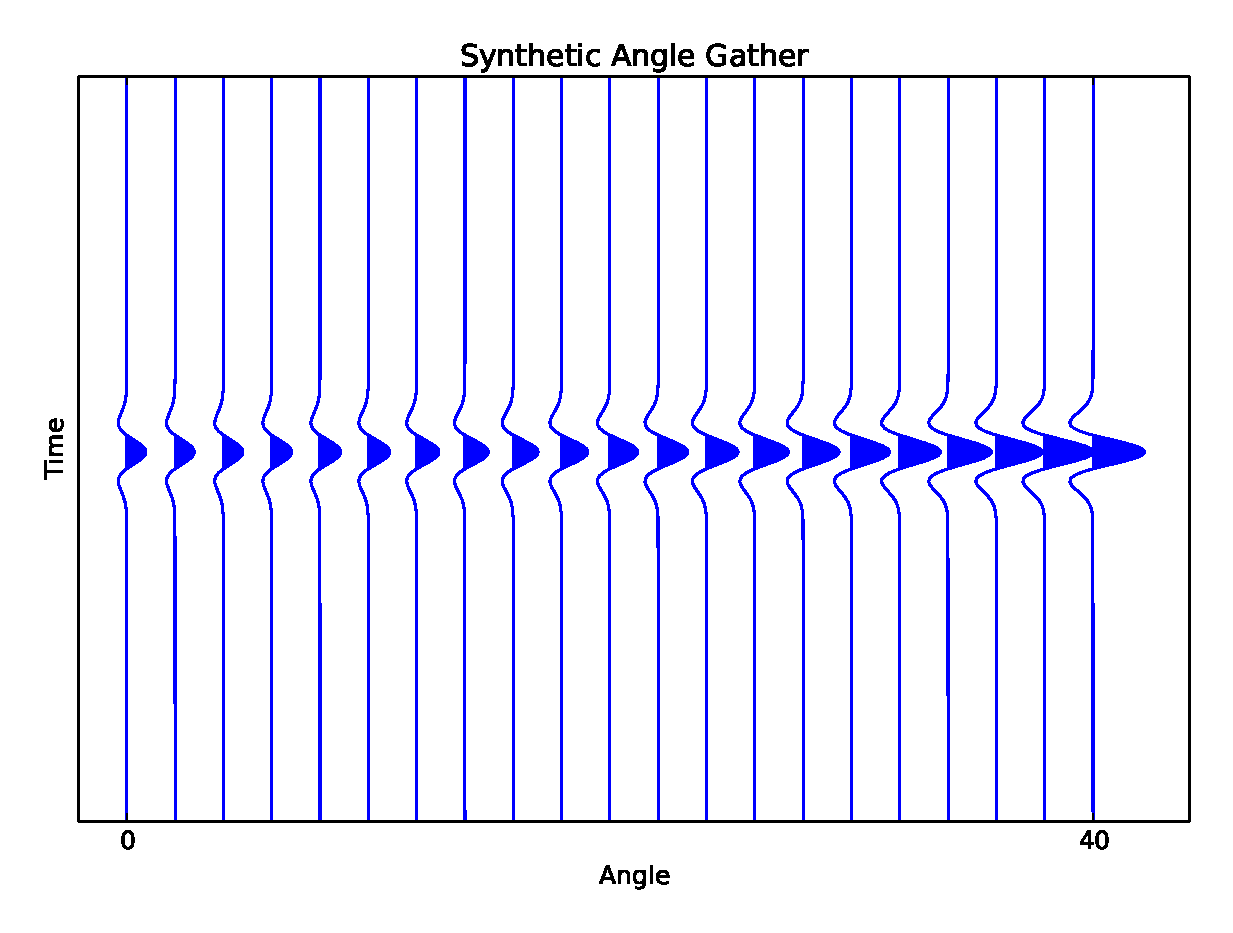
\includegraphics[scale=0.5]{wiggles.eps}
\end{center}
\end{figure}
% \caption{Well log image with stratigraphic labels.}
% \label{fig:log}
% \end{figure}





\subsubsection*{References}

\small{
Modelling of linearized Zoeppritz approximations, Arnim B. Haase 

http://www.crewes.org/ForOurSponsors/ResearchReports/2004/2004-61.pdf
\\ 
GitHub repository https://github.com/ben-bougher/geoComputing 
}

\end{document}
